
\chapter{Stochastic Calculus}

In the previous chapter the Fokker--Planck equation provided a macroscopic, deterministic description of a stochastic process: deterministic not in the trajectories, but in the probability density, which evolves according to an ordinary partial differential equation.
We now look at the same physics from the complementary point of view of the \emph{trajectory} itself, encoded in a stochastic differential equation of the Langevin type.
The two descriptions turn out to be perfectly equivalent --- and we will build the dictionary between them --- but giving a precise meaning to the equation of the trajectory is surprisingly subtle.
The culprit is a fact we proved in Chapter~3: the trajectories of the Wiener process are nowhere differentiable.
Making sense of a ``differential equation'' for a non-differentiable function forces us to construct a new calculus --- \emph{stochastic calculus} --- in which the ordinary rules of differentiation no longer hold, and to replace them with It\^o's rules.
By the end of the chapter we will be solving stochastic differential equations as comfortably as ordinary ones, including the two that dominate quantitative finance: geometric Brownian motion and the Ornstein--Uhlenbeck process.


\section[From the Fokker--Planck equation to the Langevin equation]
{From the Fokker--Planck equation to the\\Langevin equation}

Two questions guide this section.
First, in what sense is the Fokker--Planck equation equivalent to a Langevin-type stochastic differential equation (SDE) for the trajectory?
Second, what exactly is the relation between the \emph{white noise} $\xi(t)$ that appears in the Langevin equation and the Wiener process $W(t)$ of the previous chapter?

Recall the Langevin equation of Chapter~2,
\begin{equation}
\frac{dv}{dt} = -\gamma v + \xi(t),\qquad \gamma := \frac{6\pi\eta R}{m},
\end{equation}
which described the velocity of a Brownian particle subject to viscous damping and to a random force.
We now promote it to the general form
\begin{equation}
\frac{dx(t)}{dt} = a + b\,\xi(t),\qquad a\in\mathbb{R},\ b\in\mathbb{R}^+,
\end{equation}
where the constants $a$ and $b$ will turn out to be directly connected to the coefficients $a_1,a_2$ of the Fokker--Planck equation.

First we must say what we mean by the noise.
Here $\xi$ denotes normalized Gaussian white noise, a generalized random process rather than a function with pointwise values.
Its covariance formulas are interpreted distributionally; its amplitude need not equal that of the physical random force in Chapter~2.
It has three formal properties:
\begin{enumerate}[label=(\roman*)]
    \item it has zero mean, $\langle\xi(t)\rangle = 0$ for all $t$;
    \item it is delta-correlated, $\langle\xi(t)\xi(t')\rangle = \delta(t-t')$ for all $t,t'$: the noise at two distinct instants, however close, is completely uncorrelated;
    \item $\xi(t)$ is Gaussian.
    % CLAUDE NOTE: in the handwritten notes property (iii) carries a "(?)" next to "gaussiano".
    % Properties (i)-(ii) already suffice to compute <x(t)> and Var[x(t)]; gaussianity is the
    % extra hypothesis that turns "uncorrelated" into "independent".
\end{enumerate}
Properties (i) and (ii) are enough for everything we compute in this section; the third is needed because uncorrelated variables are independent only in the Gaussian case, and independence is what we will eventually use.
The name ``white'' comes from the flat power spectrum implied by (ii): all frequencies contribute equally, like white light.

Let us see what this SDE predicts.
Integrating,
\begin{equation}
dx(t) = a\,dt + b\,\xi(t)\,dt \implies x(t) = x(0) + a\int_0^t dt' + b\int_0^t \xi(t')\,dt'.
\end{equation}
Taking the ensemble average and using property (i),
\begin{equation}
\mathbb{E}[x(t)] = \langle x(0)\rangle + a\int_0^t dt' + b\int_0^t \langle\xi(t')\rangle\,dt' = \langle x(0)\rangle + a\,t,
\end{equation}
which coincides with the Fokker--Planck result $\langle x(t)\rangle = \langle x(0)\rangle + v\,t$ provided we identify $a=v=a_1$: the coefficient $a$ is the \emph{drift}.
For the second moment, squaring the solution and averaging,
\begin{equation}
\mathbb{E}[x^2(t)] = \langle x^2(0)\rangle + 2a\,t\,\langle x(0)\rangle + a^2 t^2 + b^2\int_0^t dt'\int_0^t dt''\,\underbrace{\langle\xi(t')\xi(t'')\rangle}_{\delta(t'-t'')},
\end{equation}
and since the double integral collapses on the diagonal, $\int_0^t dt'\int_0^t dt''\,\delta(t'-t'') = t$, we find
\begin{equation}
\mathrm{Var}[x(t)] = \mathbb{E}[x^2(t)] - \mathbb{E}^2[x(t)] = \mathrm{Var}[x(0)] + b^2 t.
\end{equation}
Comparing with the Fokker--Planck result $\mathrm{Var}[x(t)] = \mathrm{Var}[x(0)] + D\,t$, we identify $b^2 = D = a_2$: the squared noise amplitude is the \emph{diffusion} coefficient.

This establishes the dictionary between the Fokker--Planck equation and the (It\^o) SDE:
\begin{equation}
a_1(x,t)\ \longleftrightarrow\ a(x,t),\qquad a_2(x,t)\ \longleftrightarrow\ b^2(x,t).
\end{equation}
Explicitly: given the SDE $\dfrac{dx(t)}{dt} = a(x,t) + b(x,t)\,\xi(t)$, with $\langle\xi(t)\rangle=0$ and $\langle\xi(t)\xi(t')\rangle=\delta(t-t')$, the associated Fokker--Planck equation is
\begin{equation}
\frac{\partial}{\partial t}P(x,t) = -\frac{\partial}{\partial x}\big[a(x,t)P(x,t)\big] + \frac{1}{2}\frac{\partial^2}{\partial x^2}\big[b^2(x,t)P(x,t)\big],
\end{equation}
and, conversely, given the Fokker--Planck equation
\begin{equation}
\frac{\partial}{\partial t}P(x,t) = -\frac{\partial}{\partial x}\big[a_1(x,t)P(x,t)\big] + \frac{1}{2}\frac{\partial^2}{\partial x^2}\big[a_2(x,t)P(x,t)\big],
\end{equation}
the equivalent SDE is
\begin{equation}
\frac{dx(t)}{dt} = a_1(x,t) + \sqrt{a_2(x,t)}\,\xi(t),\qquad \langle\xi(t)\rangle=0,\ \langle\xi(t)\xi(t')\rangle=\delta(t-t').
\end{equation}
The macroscopic and the microscopic descriptions carry exactly the same information, and one can move freely between them.

There is, however, a difficulty --- and it is not a pedantic one: what we have just written is, strictly speaking, meaningless.
Take the Wiener process itself, with $a_1(x,t)=0$ and $a_2(x,t)=1$; the equivalent SDE would read
\begin{equation}
\frac{dW(t)}{dt} = 0 + \xi(t),
\end{equation}
but we proved in Chapter~3 that the trajectories of $W(t)$ have \emph{no derivative} almost surely, so the left-hand side does not exist.
The noise itself is no healthier:
\begin{equation}
\mathrm{Var}[\xi(t)] = \lim_{t'\to t}\langle\xi(t)\xi(t')\rangle = \delta(0) = \infty,
\end{equation}
an object with infinite variance at every instant, which exists nowhere in nature.
Both pathologies have the same cure, to which we now turn: stop dividing by $dt$, and work directly with the increments.


\section{White noise and the Wiener differential}

To give a rigorous meaning to the formal manipulations above, we look for the precise relation between $\xi(t)$ and $W(t)$.
The starting point is the autocorrelation of the Wiener process computed in Chapter~3,
\begin{equation}
\langle W(t)W(t')\rangle = \min(t,t') = t\,\Theta(t'-t) + t'\,\Theta(t-t'),
\end{equation}
where in the second equality we have rewritten the minimum through the Heaviside step function $\Theta$ --- a form that can be differentiated.
Differentiating with respect to $t$ in the distributional sense (the derivative of $\Theta$ being a delta, whose two contributions cancel),
\begin{equation}
\frac{d}{dt}\big[t\,\Theta(t'-t) + t'\,\Theta(t-t')\big] = \Theta(t'-t),
\end{equation}
and differentiating once more, now with respect to $t'$,
\begin{equation}
\frac{d}{dt}\frac{d}{dt'}\langle W(t)W(t')\rangle = \delta(t-t') \overset{!}{=} \langle\xi(t)\xi(t')\rangle.
\end{equation}
The autocorrelation of the ``derivative'' of the Wiener process is exactly the autocorrelation of white noise.
This justifies, in the distributional sense, the two key identities on which everything else rests.
First,
\begin{equation}
\frac{dW(t)}{dt} = \xi(t),
\qquad\text{so that}\qquad
\int_0^t \xi(t')\,dt' = \int_0^t dW(t') = W(t)-W(0);
\end{equation}
white noise is the (distributional) derivative of the Wiener process, and if $\xi(t)$ is Gaussian, so is $W(t)$.
Second, at the level of increments,
\begin{equation}
\langle dW(t)\,dW(t')\rangle = \delta(t-t')\,dt\,dt' \implies \langle dW^2(t)\rangle = dt,
\end{equation}
while $\langle dW(t)\,dW(t')\rangle = 0$ for $t\ne t'$, which --- the process being Gaussian --- means full independence of increments at different times.
The scaling $\langle dW^2\rangle = dt$ is the single most consequential formula of this chapter; we will meet it again as $[dW]^2=dt$.

The practical moral is this: the ill-defined product $b\,\xi(t)\,dt$ must everywhere be replaced by the perfectly well-defined \emph{Wiener differential} $b\,dW(t)$,
\begin{equation}
dx(t) = a\,dt + b\,\xi(t)\,dt \quad\longrightarrow\quad dx(t) = a\,dt + b\,dW(t).
\end{equation}
No derivative of $W$ ever appears; only its increments do, and those are honest Gaussian random variables.


\section{The stochastic integral}

Having agreed to write SDEs in differential form, we must say what it means to \emph{integrate} them.

\medskip
\noindent\textbf{Definition.}
Let $x(t)$ be a stochastic process; the associated SDE is
\begin{equation}
dx(t) = a(x,t)\,dt + b(x,t)\,dW(t)
\end{equation}
(an abbreviated notation: $dW(t)$ standing alone is meaningless), and for every $t$ it holds that
\begin{equation}
x(t) = x(t_0) + \int_{t_0}^{t} a(x,t')\,dt' + \underbrace{\int_{t_0}^{t} b(x,t')\,dW(t')}_{\text{stochastic integral}}.
\end{equation}
\medskip

The first integral is an ordinary one; all the novelty sits in the second, the \emph{stochastic integral}, in which the integration variable is itself a random process.
One can show that this integral exists and is unique --- but, as we are about to discover, only after one extra choice has been made.

Let $G(t)$ be the integrand and ask: what is the meaning of $\displaystyle\int_{t_0}^{t} G(t')\,dW(t')$?
We proceed as Riemann taught us, by discretization.
Partition $[t_0,t]$ into small intervals $[t_{i-1},t_i]$, choose in each an evaluation point $\tau_i\in[t_{i-1},t_i]$, and form the Riemann--Stieltjes-like sum
\begin{equation}
S_m = \sum_{i=1}^{m} G(\tau_i)\big\{W(t_i)-W(t_{i-1})\big\}.
\end{equation}
To see whether the choice of $\tau_i$ matters --- for an ordinary integral it would not --- take as a probe the simplest non-trivial integrand, $G(\tau_i)=W(\tau_i)$.
The average of the sum is then computable from the autocorrelation $\langle W(t)W(s)\rangle=\min(t,s)$:
\begin{equation}
\langle S_m\rangle = \sum_{i=1}^{m}\big\langle W(\tau_i)\{W(t_i)-W(t_{i-1})\}\big\rangle = \sum_{i=1}^{m}\big\{\min(\tau_i,t_i) - \min(\tau_i,t_{i-1})\big\} = \sum_{i=1}^{m}\{\tau_i - t_{i-1}\}.
\end{equation}
Parametrizing the evaluation point by its relative position in the interval,
\begin{equation}
\tau_i = \alpha\,t_i + (1-\alpha)\,t_{i-1},\qquad \alpha\in[0,1]
\qquad (\alpha=1\Rightarrow\tau_i=t_i,\quad \alpha=0\Rightarrow\tau_i=t_{i-1}),
\end{equation}
we obtain
\begin{equation}
\langle S_m\rangle = \sum_{i=1}^{m}\big\{\alpha t_i + (1-\alpha)t_{i-1} - t_{i-1}\big\} = \alpha\sum_{i=1}^{m}(t_i - t_{i-1}) = \alpha\,(t-t_0),
\end{equation}
which ranges over the whole interval $0\le\langle S_m\rangle\le t-t_0$ as $\alpha$ varies.

This is the crucial --- and disconcerting --- discovery: the value of a stochastic integral \emph{depends on where inside each interval the integrand is evaluated}.
The roughness of the Wiener path is to blame: within a single interval $[t_{i-1},t_i]$ the integrand moves by $\sim\sqrt{\Delta t}$, which is too much to be washed out in the limit.
Different choices of $\alpha$ therefore define genuinely different integrals, and two conventions have survived:
\begin{itemize}
    \item $\alpha=0$, $\tau_i=t_{i-1}$: the \emph{pre-point} rule, defining the \textbf{It\^o} integral;
    \item $\alpha=\tfrac{1}{2}$, $\tau_i=\tfrac{1}{2}(t_i+t_{i-1})$: the \emph{mid-point} rule, defining the \textbf{Stratonovich} integral.
\end{itemize}
The two conventions are inter-translatable, hence equivalent in content.
In finance one invariably uses It\^o, and for a good reason: the pre-point rule evaluates the integrand \emph{before} the increment arrives, i.e.\ it requires knowledge of the present only --- no peeking into the future, which is exactly the situation of a trader.
With It\^o understood, we write
\begin{equation}
S = \int_{t_0}^{t} G(t')\,dW(t'),
\end{equation}
where the convergence of $S_m$ to $S$ is meant as a \emph{mean-square limit},
\begin{equation}
S = \operatorname*{ms\text{-}lim}_{m\to\infty} S_m,\qquad
\langle S\rangle = \operatorname*{ms\text{-}lim}_{m\to\infty}\langle S_m\rangle,\qquad
\mathrm{Var}[S] = \operatorname*{ms\text{-}lim}_{m\to\infty}\mathrm{Var}[S_m],
\end{equation}
i.e.\ convergence both in mean and in variance, $\displaystyle\lim_{m\to\infty}\big\langle(S_m-S)^2\big\rangle = 0$.

It is worth spelling out the trade-off between the two conventions, because it explains why both survive in the literature.
For the \emph{Stratonovich} integral the standard rules of calculus (chain rule, Leibniz rule, and so on) continue to hold --- which is why physicists often prefer it --- but in the SDE $dx=a\,dt+b\,dW$ the coefficient $a$ is \emph{not} the drift of the process, which is counterintuitive.
For the \emph{It\^o} integral it is the other way around: $a$ gives the mean and $b^2$ the variance, with a transparent probabilistic meaning, but the standard rules of calculus \emph{fail}, and one needs a corrected change-of-variable formula (It\^o's formula, Section~\ref{sec:ito-formula}).
A simple correspondence rule connects the two conventions by shifting the drift, so nothing is lost either way.


\section{It\^o integrals}

Before stating It\^o's formula we collect\cite{Ito1944} the small toolbox of results about It\^o integrals that makes every later computation a few lines long.

\paragraph{Quadratic variation.}
For the Wiener increment $\Delta W = W(t)-W(s)$, we already know that $\langle\Delta W\rangle=0$ and $\mathrm{Var}[\Delta W]=\Delta t$ (where $\Delta t = t-s$, $t>s$).
We now need the statistics of the \emph{squared} increment $\Delta W^2 = [W(t)-W(s)]^2$, which will be summed over a partition to obtain quadratic variation.
Using $\langle W(t)W(s)\rangle=\min(t,s)=s$,
\begin{equation}
\mathbb{E}[\Delta W^2] = \mathbb{E}[W^2(t)] + \mathbb{E}[W^2(s)] - 2\langle W(t)W(s)\rangle = t + s - 2s = t-s = \Delta t,
\end{equation}
and, using the Gaussian moment identity $\mathbb{E}[\Delta W^4]=3\,\mathbb{E}[\Delta W^2]^2$,
\begin{equation}
\mathrm{Var}[\Delta W^2] = \mathbb{E}[\Delta W^4] - \mathbb{E}[\Delta W^2]^2 = 3\Delta t^2 - \Delta t^2 = 2\Delta t^2.
\end{equation}
Keep these two numbers in mind: the squared increment has mean of order $\Delta t$ but variance of order $\Delta t^2$ (standard deviation of order $\Delta t$).
That mismatch of orders is about to do a lot of work.

\paragraph{(a) Mean of an It\^o integral.}
The two basic examples are
\begin{equation}\begin{split}
\int_{t_0}^{t} dW(t') &= W(t)-W(t_0)\big|_{t_0=0} = W(t),\\
\int_{t_0}^{t} W(t')\,dW(t') &= \frac{1}{2}\big\{W^2(t)-W^2(t_0)\big\} - \frac{1}{2}(t-t_0).
\end{split}\end{equation}
The second result should give the reader pause: ordinary calculus would produce only the first term, $\tfrac12(W^2(t)-W^2(t_0))$, whereas the It\^o integral carries the \emph{anomalous} extra term $-\tfrac{1}{2}(t-t_0)$, with no classical counterpart.
Both integrals have zero mean:
\begin{equation}
\mathbb{E}\!\left[\int_{t_0}^t dW\right]=0,\qquad
\mathbb{E}\!\left[\int_{t_0}^t W\,dW\right] = \frac{1}{2}\mathbb{E}[W^2(t)] - \frac{1}{2}t = \frac{1}{2}t - \frac{1}{2}t = 0.
\end{equation}
This is no accident.
Take $G$ progressively measurable with respect to the Brownian filtration and satisfying $E[\int_{t_0}^t G(s)^2\,ds]<\infty$.
This is the non-anticipation and square-integrability condition used for the following mean and isometry statements.\footnote{Bj\"ork\cite{Bjork2020}, Definition~4.4, Proposition~4.8 and Corollary~4.9.
The full martingale definition is given in Section~\ref{sec:rn-girsanov}.}
Then
\begin{equation}
\mathbb{E}\!\left[\int_{t_0}^{t} G(t')\,dW(t')\right] = 0.
\end{equation}
The proof is one line and shows exactly where the pre-point rule enters: discretizing, $G_{i-1}=G(\tau_i=t_{i-1})$ and $\Delta W_i=W(t_i)-W(t_{i-1})$ are independent (the integrand is frozen \emph{before} the increment arrives), so
\begin{equation}
\mathbb{E}\!\left[\int_{t_0}^t G\,dW\right] = \operatorname*{ms\text{-}lim}_{m\to\infty}\sum_{i=1}^{m}\langle G_{i-1}\,\Delta W_i\rangle = \operatorname*{ms\text{-}lim}_{m\to\infty}\sum_{i=1}^{m}\langle G_{i-1}\rangle\,\langle\Delta W_i\rangle = 0.
\end{equation}

\paragraph{(b) Correlation of two It\^o integrals (It\^o isometry).}
For $G,H$ satisfying those same conditions,
\begin{equation}
\left\langle \int_{t_0}^{t} G(t')\,dW(t')\ \int_{t_0}^{t} H(t')\,dW(t')\right\rangle = \int_{t_0}^{t} dt'\,\langle G(t')H(t')\rangle;
\end{equation}
the cross terms $\langle G_{i-1}H_{j-1}\,\Delta W_i\,\Delta W_j\rangle$ with $i\ne j$ vanish by independence of the increments, while the diagonal terms reduce, through $\langle\Delta W_i^2\rangle=\Delta t$, to an ordinary Riemann integral.
The isometry converts the second moment of a stochastic integral into a deterministic integral --- it is the tool we will use every time we need a variance.

\paragraph{(c) Integration against the quadratic variation.}
For every non-anticipating $G(t)$,
\begin{equation}
\int_{t_0}^{t} G(t')\,[dW(t')]^2 = \int_{t_0}^{t} G(t')\,dt',\qquad\text{i.e.}\qquad [dW(t)]^2 = dt.
\end{equation}
The notation on the right expresses $d[W]_t=dt$ for the quadratic variation; it is not a pathwise equality $(W_{t+dt}-W_t)^2=dt$ for an individual finite increment.
To see why, take $G=1$; the claim amounts to $t = \operatorname*{ms\text{-}lim}_{m\to\infty} Q_m$ with $Q_m = \sum_{i=1}^{m}(\Delta W_i)^2$.
Using the two moments computed above with uniform spacing $\Delta t = t/m$,
\begin{equation}\begin{split}
\mathbb{E}[Q_m] &= \sum_{i=1}^{m}\mathbb{E}[\Delta W_i^2] = \sum_{i=1}^{m}\frac{t}{m} = t,\\
\mathrm{Var}[Q_m] &= \sum_{i=1}^{m}\mathrm{Var}[\Delta W_i^2] = \sum_{i=1}^{m} 2\frac{t^2}{m^2} = \frac{2t^2}{m} \xrightarrow{\ m\to\infty\ } 0,
\end{split}\end{equation}
so the mean of $Q_m$ is already exactly $t$, and its fluctuations die out as $m\to\infty$: $\big\langle(Q_m-t)^2\big\rangle = \mathrm{Var}[Q_m]\to0$, which is precisely $\operatorname*{ms\text{-}lim}Q_m = t$.
Each individual $(\Delta W_i)^2$ is random, but their sum self-averages.
As a corollary of the same order counting, $dW(t)\,dt = 0$ and $[dW(t)]^{2+N}=0$ for every $N>0$: in stochastic calculus, $dW$ behaves as an object of order $\sqrt{dt}$, and only the combinations $dt$ and $dW^2$ survive at first order.


\section{It\^o's formula}
\label{sec:ito-formula}

The fact that $[dW]^2=dt$ is of \emph{first} order in $dt$ has a dramatic consequence: the chain rule of ordinary calculus must be modified.
The corrected rule is \emph{It\^o's formula} (It\^o's lemma), the change-of-variable formula of stochastic calculus, and it is the single most used result in mathematical finance.

Let $x(t)$ obey the It\^o SDE
\begin{equation}
dx(t) = a(x,t)\,dt + b(x,t)\,dW(t),
\end{equation}
and consider a smooth function $f[x(t)]$ of the process --- for instance $f=\log x(t)$, the function that turns prices into returns.
Since $dW\sim\sqrt{dt}$, a first-order Taylor expansion is not enough: the second-order term contains $(dx)^2\supset b^2\,dW^2 = b^2\,dt$, which is of the same order as the first-order drift.
We must therefore expand to second order,
\begin{equation}
df[x(t)] = f[x(t)+dx(t)] - f[x(t)] = \frac{\partial f}{\partial x}\,dx + \frac{1}{2}\frac{\partial^2 f}{\partial x^2}\,(dx)^2,
\end{equation}
where, by the multiplication table of the previous section,
\begin{equation}
(dx)^2 = a^2\,dt^2 + 2ab\,dW\,dt + b^2\,dW^2 = b^2\,dt,
\end{equation}
because $dt^2$ and $dW\,dt$ vanish while $dW^2 = dt$.
Collecting terms, and allowing $f$ to depend explicitly on time as well, $f=f(x,t)$, we obtain
\begin{equation}
df(x,t) = \left[\frac{\partial f}{\partial t} + a(x,t)\frac{\partial f}{\partial x} + \frac{1}{2}b^2(x,t)\frac{\partial^2 f}{\partial x^2}\right]dt + b(x,t)\frac{\partial f}{\partial x}\,dW(t).
\label{eq:ito-formula}
\end{equation}
This is It\^o's formula.
Compared with the ordinary chain rule, it contains one intruder: the term $\tfrac{1}{2}b^2\,\partial^2_x f$, the \emph{anomalous It\^o term}, through which the noise leaks into the deterministic drift of any nonlinear function of the process.
Stopping at second order is not an approximation but an exact statement in the mean-square sense, because $dt\,dW(t)\overset{\text{ms-lim}}{=}0$ and $dt^2\to0$: no higher term survives.
Whenever in the following chapters we ``apply It\^o's lemma'', it is equation~\eqref{eq:ito-formula} that is being invoked.


\section{Solving the main stochastic differential equations}

Armed with It\^o's formula, we can now solve, one by one, the stochastic differential equations that will accompany us for the rest of the book.
The strategy is always the same: find a change of variables that removes the awkward part of the equation, integrate, and translate back.

\subsection{The Wiener process}

The simplest SDE of all is
\begin{equation}
dx(t) = dW(t),\qquad (a=0,\ b=1).
\end{equation}
Integrating, $\int_0^t dx(t') = \int_0^t dW(t') = W(t)-W(0)$, so that (with $x(0)$ almost surely fixed)
\begin{equation}
x(t) = x(0) + W(t):
\end{equation}
the process is simply a Wiener process shifted by the initial condition.
Its mean is inherited unchanged,
\begin{equation}
\mathbb{E}[x(t)] = x(0),\qquad \mathbb{E}\!\left[\int_0^t dW\right]=0,
\end{equation}
while for the second moment,
\begin{equation}
\mathbb{E}[x^2(t)] = \langle x(0)x(0)\rangle + 2\langle x(0)\rangle\underbrace{\Big\langle\!\int_0^t dW(s)\Big\rangle}_{0} + \Big\langle\!\int_0^t dW(t')\!\int_0^t dW(s)\Big\rangle = x^2(0) + t,
\end{equation}
where the last term used the It\^o isometry with $G=H=1$.
Therefore
\begin{equation}
\mathrm{Var}[x(t)] = \mathrm{Var}[x(0)] + t,
\end{equation}
in agreement with the Fokker--Planck computation of Chapter~3.
For $x(0)=0$ the density solves $\partial_t P = \tfrac{1}{2}\partial^2_x P$, giving once more the familiar Gaussian
\begin{equation}
P(x,t) = \frac{1}{\sqrt{2\pi t}}\,e^{-\frac{x^2}{2t}}.
\end{equation}
The SDE form has a practical virtue that the Fokker--Planck form lacks: it can be \emph{simulated} directly.
Introducing a time slicing $dt=T/N$, the increments of $W(t)$ are generated as
\begin{equation}
dW(t) = \varepsilon\sqrt{dt},\qquad \varepsilon\sim\mathcal{N}(0,1),
\end{equation}
one independent Gaussian draw per step; iterating produces a Monte Carlo trajectory, and an ensemble of such trajectories reconstructs the density.
Figure~\ref{fig:wiener-sim} shows the result: three hundred simulated paths fanning out within the $\pm\sqrt{t}$ envelope, with the histogram of the endpoints reproducing the Gaussian $\mathcal{N}(0,T)$.
This is the bridge between the microscopic (trajectory) and macroscopic (density) descriptions made algorithmic.

% Figure generated from raw notes page 7 by images/code_for_images/wiener_ensemble.py
\begin{figure}[h!]
\centering
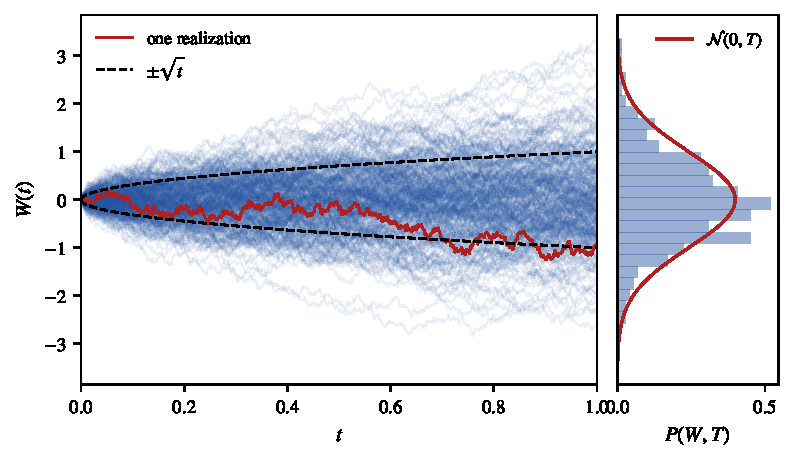
\includegraphics[width=0.9\textwidth]{images/wiener_ensemble.pdf}
\caption{Monte Carlo simulation of $300$ Wiener trajectories ($dW=\varepsilon\sqrt{dt}$, $\varepsilon\sim\mathcal{N}(0,1)$), spreading as $\sqrt{t}$ (dashed envelope). Right: histogram of the endpoints $W(T)$ against the exact density $\mathcal{N}(0,T)$. Generated by \texttt{images/code\_for\_images/wiener\_ensemble.py}.}
\label{fig:wiener-sim}
\end{figure}

\subsection{Arithmetic Brownian motion (Bachelier)}

Adding a constant drift produces the \emph{generalized Wiener process}, or arithmetic (additive) Brownian motion, with It\^o SDE\cite{Bachelier1900}
\begin{equation}
dx(t) = a\,dt + b\,dW(t),\qquad b\in\mathbb{R}^+,\ a\in\mathbb{R},
\end{equation}
called additive because the increments add up iteratively.
Integrating and taking moments exactly as before,
\begin{equation}
\mathbb{E}[x(t)] = a\,t \ \Longrightarrow\ a\ \text{is the drift},\qquad
\mathbb{E}[x^2(t)] = a^2 t^2 + b^2 t \ \Longrightarrow\ \mathrm{Var}[x(t)] = b^2 t,
\end{equation}
with standard deviation $\mathrm{s.d.}[x(t)] = b\sqrt{t}$ --- the quantity that finance calls the \emph{volatility} --- and the full distribution is Gaussian at all times,
\begin{equation}
\mathrm{PDF}(x,t) = \mathcal{N}(a\,t,\ b^2 t).
\end{equation}
A sample path is sketched in Figure~\ref{fig:abm}: the trajectory rattles around the straight line $\langle x(t)\rangle = a\,t$, with excursions that grow like $\sqrt{t}$.

\begin{figure}[h!]
\centering
\begin{tikzpicture}[scale=1.0]
  \draw[->] (-0.2,0) -- (7.2,0) node[right]{$t$};
  \draw[->] (0,-1.0) -- (0,2.6) node[above]{$x(t)$};
  % mean line <x(t)> = a t
  \draw[dashed,thick] (0,0) -- (6.8,2.2) node[right]{$\langle x(t)\rangle = a\,t$};
  % a jagged sample path fluctuating around the mean
  \draw[thick,blue!60!black] (0,0)
     -- (0.4,0.25) -- (0.8,0.05) -- (1.2,0.5) -- (1.6,0.35) -- (2.0,0.8)
     -- (2.4,0.55) -- (2.8,1.05) -- (3.2,0.8) -- (3.6,1.25) -- (4.0,1.0)
     -- (4.4,1.55) -- (4.8,1.3) -- (5.2,1.8) -- (5.6,1.55) -- (6.0,2.1)
     -- (6.4,1.85) -- (6.8,2.35);
\end{tikzpicture}
\caption{Arithmetic Brownian motion: a sample path fluctuating around the linear mean $\langle x(t)\rangle = a\,t$.}
\label{fig:abm}
\end{figure}

This was, in fact, the very first mathematical model of stock prices, proposed by Bachelier in his 1900 thesis\cite{Bachelier1900} --- five years before Einstein's paper on Brownian motion.
Historically glorious, but as a price model it has a fatal flaw: since the Gaussian has unbounded support and the fluctuations grow in probability, there is a nonzero probability that the price becomes \emph{negative}, which is not admissible for a stock.
Its autocovariance, for the record, is
\begin{equation}
\mathrm{Cov}[x(t),x(s)] = \mathbb{E}[x(t)x(s)] - \mathbb{E}[x(t)]\mathbb{E}[x(s)] = b^2\langle W(t)W(s)\rangle = b^2\min(t,s).
\end{equation}
Note that so far we have not needed It\^o's formula at all: with constant coefficients, everything is linear.
The next example is where the new calculus earns its keep.

\subsection{Multiplicative linear noise}

Consider now an It\^o process in which the noise enters \emph{multiplicatively}, proportional to the process itself,
\begin{equation}
dx(t) = b\,x(t)\,dW(t) \ \Longrightarrow\ \frac{dx(t)}{x(t)} = b\,dW(t) \ne d\ln x(t),
\end{equation}
and the inequality on the right is the whole point: in ordinary calculus $dx/x$ \emph{would} equal $d\ln x$, but here it does not, and It\^o's formula tells us by how much it fails.
Take $f(x)=\ln x$ (with $x(0)>0$); applying~\eqref{eq:ito-formula} with $a=0$, $\partial_x f = 1/x$ and $\partial_x^2 f = -1/x^2$,
\begin{equation}
d\ln x(t) = \left[\,0\cdot\frac{1}{x} + \frac{1}{2}b^2 x^2\left(-\frac{1}{x^2}\right)\right]dt + b\,x\,\frac{1}{x}\,dW(t) = -\frac{b^2}{2}\,dt + b\,dW(t).
\end{equation}
The anomalous term has generated a \emph{negative drift} $-b^2/2$ out of pure noise.
In logarithmic variables the process is now simple --- an additive Brownian motion --- with
\begin{equation}
\mathbb{E}[\ln x(t)] = \ln x_0 - \frac{b^2}{2}\,t,\qquad \mathrm{Var}[\ln x(t)] = b^2 t.
\end{equation}
Integrating and exponentiating back,
\begin{equation}
\ln x(t) = \ln x(0) - \frac{b^2}{2}\,t + b\,W(t) \ \Longrightarrow\ x(t) = x_0\,\exp\!\left\{-\frac{b^2}{2}\,t + b\,W(t)\right\},
\end{equation}
which is manifestly positive at all times.
One more check is instructive.
Setting $z=\ln x(t)\sim\mathcal{N}\!\big(\ln x_0-\tfrac{b^2}{2}t,\,b^2 t\big)$ and using the Gaussian identity $\langle e^{z}\rangle = e^{\langle z\rangle + \frac{1}{2}\mathrm{Var}[z]}$,
\begin{equation}\begin{split}
\mathbb{E}[x(t)] = \langle e^{z}\rangle &= e^{\,\langle z\rangle + \frac{1}{2}\mathrm{Var}[z]}\\
&= e^{\ln x_0 - \frac{b^2}{2}t}\,e^{\frac{b^2}{2}t} = x_0.
\end{split}\end{equation}
The two effects cancel exactly: the anomalous drift pushes the \emph{typical} trajectory down, while the fat upper tail of the exponential pulls the \emph{mean} up, and the mean is preserved despite the multiplicative noise.
This tug-of-war between median and mean is a recurring theme in finance.

\paragraph*{Geometric Brownian motion.}

Adding a linear drift to the multiplicative noise gives the \emph{geometric Brownian motion} (GBM), with It\^o SDE
\begin{equation}
dx(t) = a\,x(t)\,dt + b\,x(t)\,dW(t),\qquad b>0,\ a\in\mathbb{R},
\end{equation}
which is best read after dividing by $x$: the \emph{percentage} change $\dfrac{dx(t)}{x(t)} = a\,dt + b\,dW(t)$ is an arithmetic Brownian motion.
Percentage changes, not absolute ones, are what investors actually care about --- a 1\,\euro{} move means something very different for a 10\,\euro{} stock and a 1000\,\euro{} one --- and this is the economic rationale for the multiplicative structure.
By It\^o's formula, exactly as in the previous subsection but keeping the drift,
\begin{equation}
d\ln x(t) = \left(a - \frac{b^2}{2}\right)dt + b\,dW(t),
\end{equation}
so the increments $\ln\!\big(x(t+dt)/x(t)\big)$ --- the \emph{log-returns} --- are Gaussian, and the arithmetic Brownian motion of the logarithm becomes the geometric motion of the price.
As before,
\begin{equation}
\mathbb{E}[\ln x(t)] = \ln x(0) + \left(a-\frac{b^2}{2}\right)t,\qquad \mathrm{Var}[\ln x(t)] = b^2 t,
\end{equation}
\begin{equation}
\mathrm{PDF}(\ln x(t),t) = \mathcal{N}\!\left(\ln x_0 + \Big(a-\frac{b^2}{2}\Big)t,\ b^2 t\right),
\end{equation}
and translating back to the price itself,
\begin{equation}
\mathbb{E}[x(t)] = x_0\,e^{at},\qquad \mathrm{Var}[x(t)] = x_0^2\,e^{2at}\big(e^{b^2 t}-1\big).
\end{equation}
The process never becomes negative and its mean grows exponentially at rate $a$, which makes GBM a \emph{plausible model for spot prices} --- indeed, the standard one, as we will see at length in the next chapter.
It was introduced in finance by Osborne in 1959\cite{Osborne1959}, and was later given a proper economic rationale by Samuelson (1965)\cite{Samuelson1965}.
% CLAUDE NOTE: the notes cite "Samuelson 1960"; corrected to 1965 in the text at the
% author's request (2026-07-02). The reference is Samuelson's "Rational Theory of
% Warrant Pricing", Industrial Management Review 6 (1965).
Since the model is Markovian, the prices before $x(0)$ are irrelevant to the future --- an assumption still debated, to which we return in Chapter~5.

\subsection{The Ornstein--Uhlenbeck process}

Our last and richest example is the \emph{Ornstein--Uhlenbeck} (OU) process.
It occupies a special place in the theory: by \emph{Doob's theorem}\cite{Doob1942,UhlenbeckOrnstein1930} under the usual nondegeneracy and regularity assumptions it characterizes the stationary scalar Gaussian Markov case (in the strong sense, $P_t(x,t)=P_t(x)$).
Uniqueness makes it the default model for any quantity that fluctuates around a stable level: short-term interest rates, volatility, or the velocity of a Brownian particle.
Its It\^o SDE is
\begin{equation}
dx(t) = -\kappa\,x\,dt + \sqrt{D}\,dW(t),\qquad \kappa>0,\ [\kappa]=T^{-1},\ \tau=\frac{1}{\kappa},
\end{equation}
a random walk tethered by a linear restoring force: whenever $x$ wanders away from zero, the drift $-\kappa x$ pulls it back, on the characteristic time scale $\tau=1/\kappa$.

To solve it we use the substitution $f(x,t)=x\,e^{\kappa t}$ (an integrating factor), designed precisely to absorb the restoring drift.
By It\^o's formula,
\begin{equation}
df(x,t) = \left[\frac{\partial f}{\partial t} + a\frac{\partial f}{\partial x} + \frac{1}{2}b^2\frac{\partial^2 f}{\partial x^2}\right]dt + b\frac{\partial f}{\partial x}\,dW(t) = \sqrt{D}\,e^{\kappa t}\,dW(t),
\end{equation}
because the two drift contributions cancel identically ($\kappa x e^{\kappa t} - \kappa x e^{\kappa t}=0$) and $f$ is linear in $x$, so no anomalous term appears.
What remains is a pure (time-modulated) noise, which we integrate at sight:
\begin{equation}
\int_0^t df(x(t'),t') = \sqrt{D}\int_0^t e^{\kappa t'}\,dW(t'),
\end{equation}
and since $x(t)=f\,e^{-\kappa t}$ with $x(0)$ almost surely fixed,
\begin{equation}
x(t) = x_0\,e^{-\kappa t} + \sqrt{D}\int_0^t e^{-\kappa(t-t')}\,dW(t').
\end{equation}
The structure is transparent: the initial condition decays exponentially, while the noise accumulates --- but each past kick $dW(t')$ is remembered only with the fading weight $e^{-\kappa(t-t')}$.
Taking the mean (the It\^o integral averages to zero),
\begin{equation}
\mathbb{E}[x(t)] = x_0\,e^{-\kappa t},
\end{equation}
and, computing the variance with the It\^o isometry,
\begin{equation}\begin{split}
\mathrm{Var}[x(t)] = \Big\langle\big(x(t)-\langle x(t)\rangle\big)^2\Big\rangle &= D\,e^{-2\kappa t}\int_0^t \big(e^{\kappa t'}\big)^2\,dt'\\
&= D\,e^{-2\kappa t}\,\frac{e^{2\kappa t}-1}{2\kappa} = \frac{D}{2\kappa}\big(1-e^{-2\kappa t}\big).
\end{split}\end{equation}

The two limiting regimes are revealing.
For long times, $t\gg1/\kappa$, the memory of the initial condition is gone and the variance saturates,
\begin{equation}
\mathbb{E}[x(t)]\to0,\qquad \mathrm{Var}[x(t)]\to\frac{D}{2\kappa},
\end{equation}
so the distribution converges to a stationary law; a process initialized with fixed $x_0$ is not stationary at finite times: the injection of noise ($D$) and the dissipation of the restoring force ($\kappa$) balance.
For short times, $t\ll1/\kappa$, expanding the exponentials gives
\begin{equation}
\mathbb{E}[x(t)]\to x_0\{1-\kappa t+\dots\},\qquad \mathrm{Var}[x(t)]\to\frac{D}{2\kappa}\{1-1+2\kappa t+\dots\} = D\,t,
\end{equation}
i.e.\ before the restoring force has had time to act, the process simply \emph{diffuses} like a free Brownian motion.
The full distribution at all times is Gaussian,
\begin{equation}
\mathcal{N}\!\left(x_0\,e^{-\kappa t},\ \frac{D}{2\kappa}\big[1-e^{-2\kappa t}\big]\right) \xrightarrow{\ t\to\infty\ } \mathcal{N}\!\left(0,\ \frac{D}{2\kappa}\right) = P^{\mathrm{O.U.}}(x).
\end{equation}
In the original physical setting, where $x$ is the velocity of a Brownian particle, the stationary law $P^{\mathrm{O.U.}}(v) = P^{\mathrm{M.B.}}(v)$ is nothing but the Maxwell--Boltzmann distribution: the OU process describes, in real time, how an out-of-equilibrium velocity distribution relaxes to thermal equilibrium, and matching the two stationary variances yields the Einstein fluctuation--dissipation relation, $D/(2\kappa)=k_BT/m$ for the velocity process.
Figure~\ref{fig:ou} sketches the characteristic noisy relaxation of a single path, and Figure~\ref{fig:ou-sim} shows the full Monte Carlo picture: an ensemble of paths hugging the analytic mean, with the fluctuation band saturating at $\pm\sqrt{D/2\kappa}$.

\begin{figure}[h!]
\centering
\begin{tikzpicture}[scale=1.0]
  \draw[->] (-0.2,0.5) -- (7.2,0.5) node[right]{$t$};
  \draw[->] (0,-0.4) -- (0,2.6) node[above]{$x(t)$};
  \node[left] at (0,2.1) {$x_0$};
  % equilibrium mean level
  \node[left] at (0,0.5) {$0$};
  % damped, noisy relaxation toward the level
  \draw[thick,red!60!black] (0,2.1)
    -- (0.4,1.7) -- (0.8,1.9) -- (1.2,1.4) -- (1.6,1.55) -- (2.0,1.1)
    -- (2.4,1.25) -- (2.8,0.85) -- (3.2,1.0) -- (3.6,0.7) -- (4.0,0.8)
    -- (4.4,0.55) -- (4.8,0.65) -- (5.2,0.5) -- (5.6,0.6) -- (6.0,0.45)
    -- (6.4,0.55) -- (6.8,0.5);
\end{tikzpicture}
\caption{Ornstein--Uhlenbeck process: a noisy, exponentially damped relaxation of $x(t)$ from $x_0$ towards the stationary level, with asymptotic variance $D/2\kappa$.}
\label{fig:ou}
\end{figure}

% Figure generated from raw notes page 9 by images/code_for_images/ou_ensemble.py
\begin{figure}[h!]
\centering
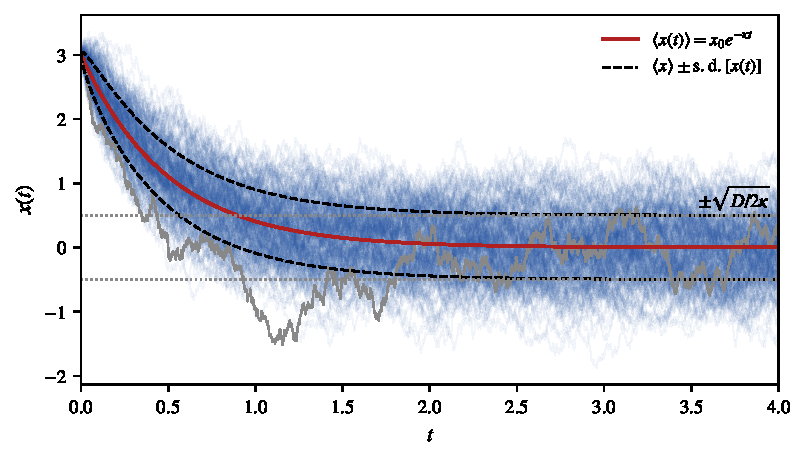
\includegraphics[width=0.9\textwidth]{images/ou_ensemble.pdf}
\caption{Monte Carlo simulation of $200$ Ornstein--Uhlenbeck paths ($\kappa=2$, $D=1$, $x_0=3$), relaxing from the common initial condition to the stationary band. The red curve is the analytic mean $x_0e^{-\kappa t}$; the dashed curves are the $\pm1$ standard-deviation envelope, saturating at $\pm\sqrt{D/2\kappa}$ (dotted). Generated by \texttt{images/code\_for\_images/ou\_ensemble.py}.}
\label{fig:ou-sim}
\end{figure}

With the Wiener process, geometric Brownian motion, and the Ornstein--Uhlenbeck process in hand, our toolbox is complete.
The next chapter puts it to work on the problem that made stochastic calculus famous: the fair pricing of financial derivatives.
